\chapter{Timestepping}
We now briefly discuss how to solve initial value problems. For more on this see Bradie~\cite[Chap. 7]{Bra06}. A slightly longer but still quick introduction to these ideas can also be found in Boyce and DiPrima~\cite{BoyDip10}.
%%%%%%%
%Section
%%%%%%%
\section{Forward Euler}
In order to compute solutions to differential equations on computers efficiently, it is convenient to do our calculations at a finite number of specified points and then interpolate between these points. For many calculations it is convenient to use a grid whose points are equally distant from each other. 

For the rest of the section $h$ will be our step size, which is assumed to be constant.  When solving an ODE or PDE, the choice of $h$ isn't selected at random, but rather requires some intuition and/or theoretical analysis. We are going to start with the forward Euler method which is the most basic numerical method. Let us first denote the time at the $n$th time-step by $t^n$ and the computed solution at the $n^{th}$ time-step by $y^n$, where $y^n \equiv y(t=t^n)$. The step size $h$ in terms of $t$ is defined as $h=t^{n+1}-t^n$. Lets first start with a basic ODE with initial conditions, in which $f(t,y)$ is some arbitrary function and $y(t)$ is our solution,
\begin{eqnarray}\label{eq:ode}
\ \frac{dy}{dt} = f(t,y) \qquad y(t^0)=y^0.
\end{eqnarray}
The differential equation can be approximated by finite differences, 
\begin{eqnarray}
\frac{y^{n+1}-y^n}{h} = f(t^n,y^n).
\end{eqnarray}
Now all we have to do is solve for $y^{n+1}$ algebraically,
\begin{eqnarray}\label{eq:odeFE}
\ y^{n+1}=y^n+h f(t^n,y^n) \qquad \text{(Forward Euler/Explicit method)}
\end{eqnarray}
If we wanted to calculate $\frac{dy}{dt}$ at time $t^0$, then we could generate an approximation for the value at time $t^{n+1}$ using \eqref{eq:odeFE} by first finding $y(t^0)$ and using it to compute $y^{n+1}$. We then repeat this process until the final time is reached.

%Subsection
\subsection{An Example Computation}
Let us consider the ODE in eq.\ \eqref{eq:ode} with $f(t,y)=y$ and initial conditions $y(t^0)=1$ where $t^0=0$. Two numerical solutions are computed using the forward Euler method with $h=1$ and $h=.1$
\begin{figure}
\begin{center}
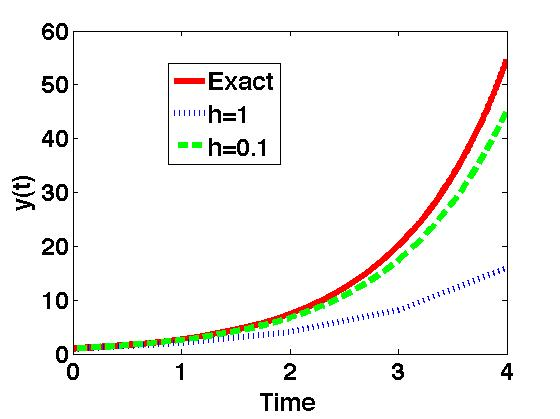
\includegraphics[scale=0.6]{./Timestepping/Forward_Euler.jpg}
\caption{A numerical solution to the ODE in eq.\ \eqref{eq:ode} with $f(t,y)=y$ demonstrating the accuracy of the Forward Euler method for different choices of timestep.} \label{fig:FEexample}
\end{center}
\end{figure}

It should be no surprise that a smaller step size like $h=.1$ compared to $h=1$ will be more accurate. Looking at the line for $h=1$, you can see that $y(t)$ is calculated at only 4 points then straight lines interpolate between each point. This is obviously not very accurate, but gives a rough idea of what the function looks like. The solution for $h=.1$ might require 10 times more steps to be taken, but it is clearly more accurate. Forward Euler is an example of a first-order method and approximates the exact solution using the first two terms in the Taylor expansion\footnote{The derivation of the Taylor expansion can be found in most books on calculus.}
\begin{eqnarray}
y(t^n+h)=y(t^n)+h \left.\frac{dy}{dt}\right|_{t^n}+\text{O}(h^2),
\end{eqnarray}
where terms of higher order than O$(h^2)$ are omitted in the approximate solution. Substituting this into eq.\ \eqref{eq:odeFE} we get that
\begin{align*}
&{} y^n +h \left.\frac{dy}{dt}\right|_{t^n}+\text{O}(h^2) = y^n +hf(t^n,y^n)
\end{align*}
after cancelling terms and dividing by $h$, we get that
\begin{align*}
&{} \left.\frac{dy}{dt}\right|_{t^n}+\text{O}(h) = f(t^n,y^n),
\end{align*}
from which it is clear that the accuracy of the method changes linearly with the step size, and hence it is first-order accurate.
%%%%%%%
%Section
%%%%%%%
\section{Backwards Euler}
A variation of forward Euler can be obtained by approximating a derivative by using a backward difference quotient. Using eq.\ \eqref{eq:ode} and applying
\begin{eqnarray}
\frac{y^{n}-y^{n-1}}{h}&\approx&f(t^n,y^n) \\
y^{n}&=&y^{n-1}+h f(t^n,y^n).
\end{eqnarray}
Stepping the index up from $n$ to $n+1$ we obtain,
\begin{eqnarray}
y^{n+1}=y^n+h f(t^{n+1},y^{n+1})\qquad \text{(Backwards Euler/Implicit method)}
\end{eqnarray}
Notice how $y^{n+1}$ is not written explicitly like it was in the forward Euler method. This equation instead implicitly defines $y^{n+1}$ and must be solved  to determine the value of $y^{n+1}$. How difficult this is depends entirely on the complexity of the function $f$. For example, if $f$ is just $y^2$, then the quadratic formula could be used, but many nonlinear PDEs require other methods. Some of these methods will be introduced later.
%%%%%%%
%Section
%%%%%%%
\section{Crank-Nicolson}
By taking an average of the forward and backward Euler methods, we can find the Crank-Nicolson method:
\begin{eqnarray}
\frac{y^{n+1}-y^{n}}{h}&=&\frac{1}{2}f(t^{n+1},y^{n+1})+\frac{1}{2}f(t^n,y^n)
\end{eqnarray}
Rearranging we obtain,
\begin{eqnarray}
y^{n+1}=y^n+\frac{h}{2}\left[ f(t^{n+1},y^{n+1})+f(t^n,y^n) \right] \qquad \text{(Crank-Nicolson)}
\end{eqnarray}
Notice again how $y^{n+1}$ is not written explicitly like it was in forward Euler. This equation instead implicitly defines $y^{n+1}$ and so the equation must be solved algebraically to obtain $y^{n+1}$. 
%%%%%%%
%Section
%%%%%%%
\section{Stability of Forward Euler, Backward Euler and Crank-Nicolson}
Let's look at the following ODE
\begin{eqnarray}
\frac{dy}{dt}= -\lambda y(t) \label{eq:ODEstability}
\end{eqnarray}
where $\lambda$ is a constant and $y(t^0)=1$ where $t^0=0$. Lets numerically solve this ODE using the forward Euler, backward Euler and Crank-Nicolson time-stepping schemes. The results are as follows
\begin{eqnarray}
y^{n+1}=y^n-\lambda h y^n \qquad \text{(Forward Euler)}\\
y^{n+1} = \frac{y^n}{(1+\lambda h)} \qquad \text{(Backward Euler)} \\
y^{n+1} = y^n\left(\frac{2-\lambda h}{2+\lambda h}\right) \qquad \text{(Crank-Nicolson)} 
\end{eqnarray}
and the exact solution is given by
\begin{eqnarray}
y(t)= e^{-\lambda t} \qquad \text{(Exact solution)}
\end{eqnarray}

\begin{figure}[h]
\begin{center}
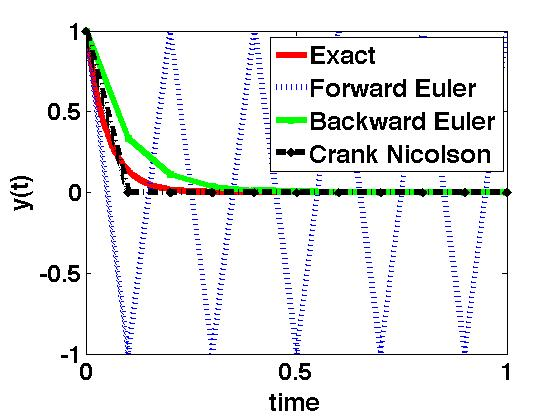
\includegraphics[scale=.4]{./Timestepping/unstable_forward_Euler.jpg}
\caption{A numerical solution to the ODE in eq.\ \eqref{eq:ODEstability} with $\lambda=20$ and with a timestep of $h=0.1$ demonstrating the instability of the Forward Euler method and the stability of the Backward Euler and Crank Nicolson methods.} \label{fig:ODEstability}
\end{center}
\end{figure}
Figure \ref{fig:ODEstability} above shows how both methods converge to the solution, but the forward Euler solution is unstable for the chosen timestep. Listing \ref{lst:MatlabInstability} is a Matlab program where you can play around with the value of $\lambda$ to see how, for a fixed timestep, this changes the stability of the method. 
\lstinputlisting[style=matlab_style,language=Matlab,label=lst:MatlabInstability,caption={A Matlab program to demonstrate instability of different timestepping methods.}]{./Timestepping/Programs/Simple_ODE_Example_of_Unstable_FE.m}

%%%%%%%
%Section
%%%%%%%
\section{Stability and Accuracy of Forward Euler, Backward Euler and Crank-Nicolson Time Stepping Schemes for $y'=-\lambda y$}

The examples discussed show that numerical stability is an important consideration when finding approximate solutions to differential equations on computers. Numerical stability requires a careful choice of numerical method and timestep for each numerical solution to a differential equation. We now try to understand these observations so that we have some guidelines to design numerical methods that are stable. The numerical solution to an initial value problem with a bounded solution is {\bf stable} if the numerical solution can be bounded by functions which are independent of the step size. There are two methods which are typically used to understand stability. The first method is linearized stability, which involves calculating eigenvalues of a linear system to see if small perturbations grow or decay. A second method is to calculate an energy like quantity associated with the differential equation and check whether this remains bounded. 

We shall assume that $\lambda\geq0$ so that the exact solution to the ODE does not grow without bound. The forward Euler method gives us
\begin{align*}
&{} \frac{y^{n+1}-y^n}{h}=-\lambda y^n
\\&{} y^{n+1}=(1-\lambda h)y^n
\\&{} \Rightarrow \lvert y^{n+1} \rvert \geq \lvert (1-\lambda h) \rvert \lvert y^n \rvert \quad \text{ if } \lvert (1-\lambda h) \rvert > 1
\\&{} \Rightarrow \lvert y^{n+1} \rvert \leq \lvert (1-\lambda h) \rvert \lvert y^n \rvert \quad \text{ if } \lvert (1-\lambda h) \rvert <1.
\end{align*}

We can do a similar calculation for backward Euler to get
\begin{align*}
&{} \frac{y^{n+1}-y^n}{h}=-\lambda y^{n+1}
\\&{} y^{n+1}=\frac{y^n}{1+\lambda h}
\\&{} \Rightarrow \lvert y^{n+1} \rvert \leq \left\lvert \frac{y^n}{1+\lambda h} \right\rvert \leq \lvert y^n \rvert \quad \text{ since } \left\lvert \frac{1}{1+\lambda h} \right\rvert <1.
\end{align*}
Thus, the backward Euler method is unconditionally stable, whereas the forward Euler method is not. We leave the analysis of the Crank-Nicolson method as an exercise.

A second method, often used to show stability for partial differential equations is to look for an energy like quantity and show that this bounds the solution and prevents it from becoming too positive or too negative. Usually, the quantity is chosen to be non negative, then all one needs to do is deduce there is an upper bound. We sketch how this is done for an ordinary differential equation so that we can use the same ideas when looking at partial differential equations. Recall that the forward Euler algorithm is given by
$$\frac{y^{n+1}-y^n}{h}=-\lambda y^n.$$
Multiplying this by $y^{n+1}$ we find that
\begin{align*}
&{} (y^{n+1})^2=(1-h\lambda)y^ny^{n+1}.
\end{align*}
Now to obtain a bound on $\lvert y^{n+1}\rvert$ in terms of $\lvert y^n \rvert$, we use the following fact
$$(a-b)^2\geq0\Rightarrow a^2+b^2\geq2ab\Rightarrow\frac{(y^{n+1})^2+(y^n)^2}{2}\geq y^ny^{n+1}.$$
Hence a sufficient condition for stability if 
$$(1-h\lambda)>0$$
is that
\begin{align*}
&{} (y^{n+1})^2\leq(1-h\lambda)\frac{(y^{n+1})^2+(y^n)^2}{2}
\\&{} (y^{n+1})^2\frac{1+h\lambda}{2}\leq\frac{1-h\lambda}{2}(y^n)^2
\\&{} (y^{n+1})^2\leq\frac{1-h\lambda}{1+h\lambda}(y^n)^2,
\end{align*}
thus if $1-h\lambda>0$, then $0<\frac{1-h\lambda}{1+h\lambda}<1$ and so we have stability, we again see that the algorithm is stable provided the timestep is small enough. There are many situations for which $\lambda$ is large and so the timestep, $h$ needs to be very small. In such a situation, the forward Euler method can be very slow on a computer.

Stability is not the only requirement for a numerical method to approximate the solution to an initial value problem. We also want to show that as the timestep is made smaller, the numerical approximation becomes better. For the forward Euler method we have that
\begin{align*}
  &{} \frac{y^{n+h}-y^{n}}{h}=-\lambda y^n
\end{align*}
now if
\begin{align*}
&{}y^n=y(t) \\
&{}y^{n+1}=y(t+h)
\end{align*}
then\footnote{We will use big `Oh' to mean that there exists a constant so that if $f~O(h)$, then for $h\rightarrow0$, we have that $\left|\frac{f}{h}\right|<C$, where $C$ is some constant.}
\begin{align*}
\\&y^{n+1}= y(t)+h\frac{\mathrm{d}y}{\mathrm{d}t} + O(h^2)
\end{align*}
so
\begin{align*}
\frac{y^{n+1}-y^n}{h}+\lambda y^n &{} = \frac{y(t+h)-y(t)}{h} +\lambda y(t)
\\&{} =\frac{\mathrm{d}y}{\mathrm{d}t} +O(h)+\lambda y(t)
\\&{} = O(h).
\end{align*}
We can do a similar calculation to show that the Crank-Nicolson method is second-order. In this case however, we use Taylor expansions around $y(t+h/2)$.
\begin{align*}
&{}\frac{y^{n+1}-y^n}{h}=-\lambda \frac{ y^{n+1} + y^n}{2}
\end{align*}
so
\begin{align*}
&{} y^{n+1} =y(t+h)=y(t+h/2)+(h/2)\frac{\mathrm{d}y}{\mathrm{d}t} +(h/2)^2\frac{1}{2}\frac{\mathrm{d}^2y}{\mathrm{d}t^2} + O(h^3)
\\&{} y^{n} =y(t)=y(t+h/2)-(h/2)\frac{\mathrm{d}y}{\mathrm{d}t} +(h/2)^2\frac{1}{2}\frac{\mathrm{d}^2y}{\mathrm{d}t^2} + O(h^3)
\end{align*}
hence
\begin{align*}
\frac{y^{n+1}-y^n}{h}+\lambda \frac{ y^{n+1} + y^n}{2} &{} =\frac{\mathrm{d}y}{\mathrm{d}t} + O(h^2) +\lambda \left[y(t+h/2)+O(h^2) \right]
\\&{} = O(h^2).
\end{align*}
Thus this is a second-order method.

%%%%%%%
%Section
%%%%%%%
\section{Exercises}
\begin{enumerate}
\item[1)] Determine the real values of $\lambda$ and timestep $h$ for which the implicit midpoint rule is stable for the ODE 
\begin{equation*}
\frac{\mathrm{d}y}{\mathrm{d}t}=-\lambda y
\end{equation*}
Sketch the stable region in a graph of $\lambda$ against timestep $h$.
\item[2)] Show that the backward Euler method is a first-order method.
\end{enumerate}

